\documentclass[preprint,11pt,sort&compress]{elsarticle}

% ---------------------------------------------------------------------------
\usepackage[utf8]{inputenc}
\usepackage[T1]{fontenc}
\usepackage[spanish,es-tabla,es-nodecimaldot,es-noshorthands]{babel}
\usepackage{lmodern,microtype}
\usepackage[margin=2.5cm]{geometry}
\usepackage{amsmath,amssymb,bm}
\usepackage{graphicx,booktabs,multirow,array}
\usepackage[labelfont=bf,font=small]{caption}
\usepackage{subcaption}
\usepackage[output-decimal-marker={,},group-separator={.},range-phrase={--},
            per-mode=symbol,detect-all]{siunitx}
\usepackage{xcolor}
\usepackage[colorlinks=true,linkcolor=blue!50!black,citecolor=blue!50!black,urlcolor=blue!50!black]{hyperref}

\graphicspath{{figuras/}}
\journal{FS3003 Métodos numéricos para EDP -- Informe final}
\biboptions{numbers,sort&compress}

\newcommand{\Pf}{P_{\mathrm{falla}}}
\newcommand{\Tc}{T_{\mathrm{crit}}}
\newcommand{\Tmax}{T_{\mathrm{máx}}}
\newcommand{\hs}{h_{\mathrm{sup}}}
\newcommand{\Tamb}{T_{\mathrm{amb}}}
\newcommand{\dd}{\,\mathrm{d}}
\renewcommand{\vec}[1]{\bm{#1}}

\abstracttitle{Resumen}
\keywordtitle{Palabras clave}
\makeatletter
\def\ps@pprintTitle{\let\@oddhead\@empty\let\@evenhead\@empty
  \def\@oddfoot{\footnotesize\itshape FS3003 Métodos numéricos para EDP -- Informe final\hfill Universidad EAFIT, 2026-2}
  \let\@evenfoot\@oddfoot}
\makeatother

\begin{document}

\begin{frontmatter}

\title{Riesgo de sobrecalentamiento de un chip con carga de trabajo incierta:
elementos finitos y cuantificación probabilística para el diseño de disipadores}

\author{Nancy Burgos}
\author{Carlos Arroyave}
\author{David Restrepo}
\address{Escuela de Ciencias Aplicadas e Ingeniería, Universidad EAFIT, Medellín, Colombia}

\begin{abstract}
El disipador de un procesador se diseña antes de conocer la carga de trabajo, de modo que
el mapa de potencia que debe evacuar es incierto. En este trabajo se estima la probabilidad
de que la temperatura máxima de un chip supere su límite cuando la activación de sus bloques
funcionales es aleatoria y espacialmente correlacionada. La temperatura se modela con la
ecuación de Helmholtz modificada en dos dimensiones y se resuelve con un programa propio de
elementos finitos que admite geometrías arbitrarias, varios materiales y condiciones de
frontera mixtas, verificado con dos soluciones manufacturadas. Las activaciones se generan
con una cópula gaussiana; gracias a la linealidad del problema, la probabilidad de falla se
calcula de forma exacta y se contrasta con Monte Carlo. Con la misma capacidad total de
enfriamiento, la probabilidad de falla de cuatro estrategias de disipación varía entre
\num{0.04} y \num{0.75}. Diseñar según la potencia media da casi la misma temperatura
esperada que diseñar según la potencia pico, pero siete veces más probabilidad de falla, y
la correlación de la carga multiplica por más de treinta el riesgo del mejor diseño. Un
análisis determinista no basta para comparar estrategias de disipación.
\end{abstract}

\begin{keyword}
elementos finitos \sep gestión térmica de chips \sep cuantificación de incertidumbre
\sep Monte Carlo \sep cópula gaussiana \sep soluciones manufacturadas
\end{keyword}

\end{frontmatter}

% =============================================================================
\section{Introducción}
\label{sec:intro}

La densidad de potencia de los circuitos integrados ha crecido más rápido que la
capacidad de evacuar el calor que producen. Desde mediados de la década de 2000 la
temperatura dejó de ser un problema exclusivo del empaquetado y pasó a condicionar la
arquitectura misma del procesador \cite{skadron2003temperature,pedram2006thermal}. La
temperatura máxima de unión de un procesador comercial suele estar entre
\SIlist{100;110}{\celsius} \cite{intel_tjmax}; por encima de ese límite el chip reduce su
frecuencia o se apaga, y la operación prolongada a alta temperatura acelera los
mecanismos de degradación \cite{pedram2006thermal}. Una consecuencia extrema de esta
restricción es el llamado \emph{silicio oscuro}: en los nodos tecnológicos recientes no es
posible mantener encendidos todos los transistores del chip al mismo tiempo sin exceder
el presupuesto de potencia, de modo que en cada instante solo una fracción de los bloques
está activa \cite{esmaeilzadeh2011dark}.

Esto tiene una implicación directa para el diseño del disipador. El disipador se diseña
una sola vez, antes de saber qué programas ejecutará el chip; en cambio, qué bloques
están encendidos en cada momento depende del programa, del sistema operativo y del
usuario. El mapa de potencia que el disipador debe evacuar no es un dato sino una
variable aleatoria. Las dos alternativas deterministas habituales tienen limitaciones
claras. Diseñar para el peor caso (todos los bloques encendidos) sobredimensiona el
sistema y, como se mostrará, no permite distinguir entre diseños que en la práctica tienen
riesgos muy distintos. Diseñar para la potencia media subestima los bloques que consumen
mucho pero se usan poco, y esconde los puntos calientes que aparecen cuando varios bloques
vecinos se activan juntos.

La modelación térmica de chips en la etapa temprana de diseño suele hacerse con modelos
compactos de red térmica como HotSpot \cite{huang2006hotspot}, que representan el chip como
una red de resistencias y capacitancias con un camino vertical hacia el disipador. Esos
modelos se evalúan normalmente con trazas de potencia concretas. En este trabajo se adopta
un enfoque complementario: se resuelve la ecuación de conducción de calor con el método de
elementos finitos y se trata la activación de los bloques como un vector aleatorio con
dependencia espacial, para estimar la \emph{probabilidad} de que la temperatura máxima
supere el límite. Esa probabilidad se usa como criterio para comparar estrategias de
disipación con la misma capacidad total de enfriamiento.

Los objetivos del proyecto son: (i) implementar un solver de elementos finitos general,
capaz de resolver el problema en geometrías arbitrarias, con varios materiales y
condiciones de frontera mixtas a partir de archivos de entrada; (ii) verificar el solver
con soluciones manufacturadas; (iii) modelar las fuentes de calor como bloques con
activación aleatoria y correlacionada; (iv) estimar la probabilidad de falla térmica de
distintas estrategias de disipación; y (v) analizar su sensibilidad a la correlación
espacial y al nivel de carga.

El artículo está organizado así. La Sección~\ref{sec:metodo} presenta el modelo físico y
probabilístico, la discretización por elementos finitos, la implementación y los métodos
para estimar la probabilidad de falla. La Sección~\ref{sec:resultados} verifica el solver y
presenta y analiza los resultados del estudio del chip, y la
Sección~\ref{sec:conclusiones} resume las conclusiones y limitaciones.

% =============================================================================
\section{Metodología}
\label{sec:metodo}

Esta sección presenta primero el modelo matemático del problema, físico y probabilístico,
y después los métodos numéricos con los que se resuelve.

\subsection{Modelo térmico bidimensional}
\label{sec:modelo}

El chip es una lámina de silicio de lado $L=\SI{10}{\milli\metre}$ y espesor
$H=\SI{0.5}{\milli\metre}$. Su cara inferior contiene los transistores, que generan
calor, y su cara superior está en contacto con el disipador a través de un material de
interfaz. En estado estacionario la temperatura cumple
$-\nabla\cdot(k\nabla T)=q$ en el volumen del chip. Como la lámina es delgada, la
temperatura casi no varía en el espesor: el número de Biot asociado a la cara superior es
$\mathrm{Bi}=\hs H/k\approx\num{0.07}<\num{0.1}$ con los valores de la
Tabla~\ref{tab:parametros}, el criterio usual para despreciar los gradientes internos
\cite{incropera2007}. Integrando la ecuación en el espesor y modelando el flujo por la cara
superior con un coeficiente de transferencia $\hs(\vec x)$ que resume todo el camino
térmico hasta el aire (interfaz, base del disipador y aletas), se obtiene el problema
bidimensional
\begin{equation}
  -\nabla\cdot\bigl(k\nabla T\bigr) + \beta(\vec x)\,\bigl(T-\Tamb\bigr) = q(\vec x)
  \quad\text{en }\Omega=(0,L)^2,
  \qquad \beta(\vec x)=\frac{\hs(\vec x)}{H},
  \label{eq:edp}
\end{equation}
donde $T$ es la temperatura promediada en el espesor, $k$ la conductividad del silicio,
$q$ la potencia volumétrica disipada y $\Tamb$ la temperatura del aire dentro del equipo.
Por los cuatro bordes laterales el chip intercambia calor por convección natural,
\begin{equation}
  -k\,\frac{\partial T}{\partial n} = h_b\,\bigl(T-\Tamb\bigr)\quad\text{en }\partial\Omega .
  \label{eq:robin}
\end{equation}

Escribiendo $f=q+\beta\Tamb$, la ecuación~\eqref{eq:edp} toma la forma
$-\nabla\cdot(k\nabla T)+\beta T=f$, que es la ecuación de \emph{Helmholtz modificada}
(o de Poisson apantallada): la ecuación de Helmholtz con número de onda imaginario. A
diferencia de la ecuación de Poisson, el término $\beta T$ hace que el efecto de una fuente
decaiga con una longitud característica $\lambda=\sqrt{k/\beta}=\sqrt{kH/\hs}$. Con los
valores de la Tabla~\ref{tab:parametros}, $\lambda\approx\SI{1.9}{\milli\metre}$, del orden
del tamaño de un bloque: el calor de un bloque se evacúa principalmente hacia arriba, cerca
de donde se genera, y la distribución espacial de $\hs$ importa. Esa es la razón física de
que la ubicación del disipador sea una variable de diseño relevante.

\begin{table}[htbp]
\centering
\caption{Parámetros físicos del modelo.}
\label{tab:parametros}
\small
\begin{tabular}{@{}llll@{}}
\toprule
Símbolo & Descripción & Valor & Fuente \\
\midrule
$L$, $H$ & Lado y espesor del chip & \SI{10}{\milli\metre}, \SI{0.5}{\milli\metre} & valores típicos \\
$k$ & Conductividad del silicio (\SI{300}{\kelvin}) & \SI{148}{\watt\per\metre\per\kelvin} & \cite{glassbrenner1964} \\
$\bar h_{\mathrm{sup}}$ & Coeficiente medio por la cara superior & \SI{2e4}{\watt\per\metre\squared\per\kelvin} & $R_{ja}\approx\SI{0.5}{\kelvin\per\watt}$ \\
$h_b$ & Convección en los bordes & \SI{10}{\watt\per\metre\squared\per\kelvin} & convección natural \cite{incropera2007} \\
$\Tamb$ & Temperatura del aire interno & \SI{40}{\celsius} & supuesto \\
$\Tc$ & Temperatura máxima de unión & \SI{100}{\celsius} & \cite{intel_tjmax} \\
\bottomrule
\end{tabular}
\end{table}

\subsection{Plano del chip y modelo de fuentes}

El chip contiene $N_b=8$ bloques funcionales $\Omega_i\subset\Omega$: cuatro núcleos, una
caché de último nivel, una GPU, un controlador de memoria y un bloque de entrada/salida
(Tabla~\ref{tab:plano} y Figura~\ref{fig:disenos}, arriba a la izquierda). Cada bloque está
encendido o apagado, y cuando está encendido disipa una potencia $P_i$ repartida
uniformemente en su volumen:
\begin{equation}
  q(\vec x;\vec A) = \sum_{i=1}^{N_b} A_i\,q_i\,\chi_{\Omega_i}(\vec x),
  \qquad q_i=\frac{P_i}{|\Omega_i|\,H},
  \qquad A_i\in\{0,1\},
  \label{eq:fuente}
\end{equation}
donde $\chi_{\Omega_i}$ es la función indicadora del bloque. Las potencias y las
probabilidades de activación $p_i=P(A_i=1)$ de la Tabla~\ref{tab:plano} son supuestos
representativos de un procesador de escritorio: los núcleos tienen la mayor densidad de
potencia, la GPU consume mucho pero se usa poco y la caché está activa casi siempre. Con
todos los bloques encendidos el chip disipa \SI{106}{\watt}.

\begin{table}[htbp]
\centering
\caption{Plano de bloques del chip. $p_i$ es la probabilidad de que el bloque esté activo.}
\label{tab:plano}
\small
\begin{tabular}{@{}lcccc@{}}
\toprule
Bloque & Tamaño [\si{\milli\metre}] & $P_i$ [\si{\watt}] & Densidad [\si{\watt\per\milli\metre\squared}] & $p_i$ \\
\midrule
Núcleos 1--4 & $2\times 2$ (c/u) & 12 (c/u) & \num{3.00} & \num{0.5} \\
Caché L3 & $9.2\times 1.6$ & 8 & \num{0.54} & \num{0.7} \\
GPU & $5.6\times 4.4$ & 40 & \num{1.62} & \num{0.3} \\
Controlador de memoria & $3.2\times 2.0$ & 6 & \num{0.94} & \num{0.6} \\
Entrada/salida & $3.2\times 2.0$ & 4 & \num{0.63} & \num{0.4} \\
\bottomrule
\end{tabular}
\end{table}

Las activaciones no son independientes: tareas que usan varios núcleos o datos
compartidos tienden a activar bloques cercanos al mismo tiempo. La dependencia se modela con
una cópula gaussiana, siguiendo el método NORTA (\emph{NORmal To Anything})
\cite{cario1997norta}. Se toma un vector latente $\vec Z\sim\mathcal N(\vec 0,\Sigma)$ con
correlación exponencial en la distancia $d_{ij}$ entre los centros de los bloques,
\begin{equation}
  \Sigma_{ij}=\exp\!\left(-\frac{d_{ij}}{\ell}\right),
  \qquad
  A_i=\mathbf 1\{Z_i>c_i\},\qquad c_i=\Phi^{-1}(1-p_i),
  \label{eq:norta}
\end{equation}
donde $\ell$ es la longitud de correlación y $\Phi$ la función de distribución normal
estándar. Así cada $A_i$ tiene exactamente la probabilidad marginal $p_i$, y bloques más
cercanos están más correlacionados. El caso $\ell\to0$ corresponde a bloques
independientes, y $\ell\to\infty$ a activaciones totalmente dependientes, en las que los
bloques se encienden en un orden fijo, de mayor a menor $p_i$. La
correlación entre las variables binarias es menor que la latente:
\begin{equation}
  \rho^{A}_{ij}=\frac{\Phi_2\!\left(-c_i,-c_j;\Sigma_{ij}\right)-p_ip_j}
  {\sqrt{p_i(1-p_i)\,p_j(1-p_j)}},
  \label{eq:rhoA}
\end{equation}
donde $\Phi_2(\cdot,\cdot;\rho)$ es la distribución normal bivariada con correlación
$\rho$. Para dos núcleos vecinos con $\ell=\SI{3}{\milli\metre}$, la correlación latente es
\num{0.449} y la de las activaciones es \num{0.297}.

\subsection{Probabilidad de falla y estrategias de disipación}

Se dice que el chip falla térmicamente si su temperatura máxima supera $\Tc$. La medida de
riesgo es
\begin{equation}
  \Pf=P\!\left(\Tmax(\vec A)>\Tc\right),\qquad
  \Tmax(\vec A)=\max_{\vec x\in\Omega}T(\vec x;\vec A).
  \label{eq:pfalla}
\end{equation}

Una estrategia de disipación es una función $\hs(\vec x)$. Para que la comparación sea
justa, todas las estrategias tienen la misma capacidad total de enfriamiento,
$\int_\Omega\hs\dd A=\bar h_{\mathrm{sup}}\,L^2$, de modo que solo cambia \emph{dónde} se
enfría y no \emph{cuánto}. Se estudian cuatro estrategias (Figura~\ref{fig:disenos}):
\begin{itemize}
\item \textbf{Uniforme:} $\hs=\bar h_{\mathrm{sup}}$, el disipador estándar.
\item \textbf{Centrado:} una placa de $6\times\SI{6}{\milli\metre}$ en el centro con
  coeficiente alto y $\hs=\num{0.5}\,\bar h_{\mathrm{sup}}$ fuera de ella. Representa un
  diseño ingenuo que enfría el centro geométrico del chip.
\item \textbf{Según potencia media:} $\hs=\num{0.5}\,\bar h_{\mathrm{sup}}+c\sum_i P_ip_i\,
  \chi_{\Omega_i}/|\Omega_i|$, es decir, enfriamiento adicional proporcional a la densidad
  de potencia \emph{esperada}.
\item \textbf{Según potencia pico:} igual, pero proporcional a la densidad de potencia con
  el bloque encendido, $P_i/|\Omega_i|$, sin ponderar por $p_i$.
\end{itemize}
En los tres diseños no uniformes la constante se elige para conservar la integral de $\hs$.

\begin{figure}[htbp]
\centering
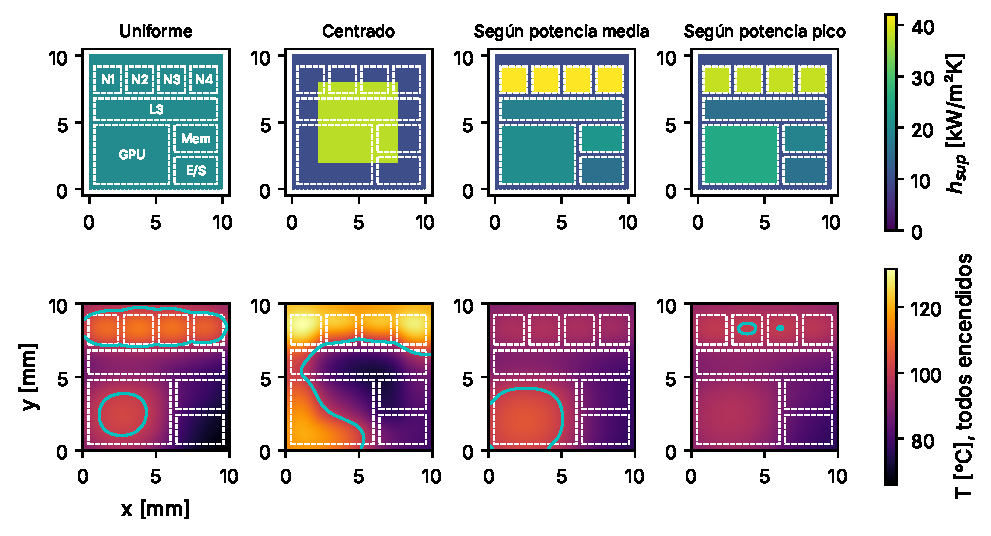
\includegraphics[width=\textwidth]{fig_disenos}
\caption{Arriba: coeficiente $\hs$ de las cuatro estrategias, todas con la misma capacidad
total de enfriamiento; las líneas discontinuas marcan los bloques (N1--N4: núcleos,
L3: caché, Mem: controlador de memoria, E/S: entrada/salida). Abajo: temperatura con
todos los bloques encendidos; la línea cian es la isoterma $\Tc=\SI{100}{\celsius}$.}
\label{fig:disenos}
\end{figure}

% =============================================================================

\subsection{Formulación débil y discretización}

El solver resuelve el problema general
\begin{equation}
\begin{aligned}
  -\nabla\cdot(k\nabla T)+\beta\,(T-T_{\mathrm{ref}}) &= q && \text{en }\Omega,\\
  T &= T_D && \text{en }\Gamma_D,\\
  k\,\partial_n T &= g && \text{en }\Gamma_N,\\
  -k\,\partial_n T &= h\,(T-T_\infty) && \text{en }\Gamma_R,
\end{aligned}
\label{eq:general}
\end{equation}
donde $k$, $\beta$, $T_{\mathrm{ref}}$ y $q$ pueden tomar valores distintos en cada
material y $\partial\Omega=\Gamma_D\cup\Gamma_N\cup\Gamma_R$. El problema del chip
\eqref{eq:edp}--\eqref{eq:robin} es el caso particular con $\Gamma_R=\partial\Omega$. Si
$V=\{v\in H^1(\Omega):v|_{\Gamma_D}=0\}$, multiplicando por $v\in V$ e integrando por
partes se obtiene la formulación débil: hallar $T$, con $T=T_D$ en $\Gamma_D$, tal que
\begin{equation}
  \int_\Omega k\nabla T\cdot\nabla v\dd\Omega
  +\int_\Omega \beta\,T v\dd\Omega
  +\int_{\Gamma_R} h\,T v\dd s
  =\int_\Omega \bigl(q+\beta T_{\mathrm{ref}}\bigr) v\dd\Omega
  +\int_{\Gamma_R} h\,T_\infty v\dd s
  +\int_{\Gamma_N} g\,v\dd s
  \qquad\forall v\in V.
  \label{eq:debil}
\end{equation}
Las condiciones de Neumann y Robin son naturales: aparecen en la forma débil y no hay que
imponerlas sobre el espacio. Como $k>0$, $\beta\ge0$ y $h\ge0$, la forma bilineal es
simétrica y coerciva siempre que haya alguna frontera de Dirichlet, de Robin con $h>0$ o un
término $\beta>0$; esto garantiza solución única \cite{larson2013fem}.

El dominio se aproxima con una malla de triángulos y $T$ con funciones lineales a trozos
(elementos P1), $T_h=\sum_j T_j\varphi_j$. Al tomar $v=\varphi_i$ se obtiene el sistema
lineal
\begin{equation}
  \bigl(\mathbf K+\mathbf M_\beta+\mathbf R\bigr)\,\mathbf T=\mathbf F+\mathbf G,
  \label{eq:sistema}
\end{equation}
con las matrices elementales, en un triángulo $e$ de área $A_e$ y una arista de frontera de
longitud $L_s$,
\begin{equation}
  \mathbf K_e=k_e A_e\,\mathbf B_e^{\!\top}\mathbf B_e,\qquad
  \mathbf M_{\beta,e}=\frac{\beta_e A_e}{12}\begin{pmatrix}2&1&1\\1&2&1\\1&1&2\end{pmatrix},\qquad
  \mathbf R_s=\frac{h_s L_s}{6}\begin{pmatrix}2&1\\1&2\end{pmatrix},
  \label{eq:elementales}
\end{equation}
donde $\mathbf B_e$ contiene los gradientes constantes de las funciones de forma. Las
matrices se obtienen simbólicamente con SymPy \cite{meurer2017sympy}, mapeando cada
triángulo al de referencia, y se convierten en funciones vectorizadas que las evalúan en
todos los elementos a la vez. El vector $\mathbf G$ reúne las contribuciones de Robin,
Neumann y del término $\beta T_{\mathrm{ref}}$. Para cargas que dependen de la posición,
$\mathbf F$ se integra con la regla de los puntos medios de las aristas, exacta para
polinomios de grado dos. Las condiciones de Dirichlet se imponen por levantamiento:
separando los nodos libres $L$ de los fijos $D$, se resuelve
$\mathbf A_{LL}\mathbf T_L=\mathbf b_L-\mathbf A_{LD}\mathbf T_D$.

La matriz se ensambla en formato disperso y se factoriza una sola vez con una
descomposición LU dispersa (SuperLU, a través de SciPy \cite{virtanen2020scipy}). En la
malla del chip de $100\times100$ celdas (\num{10201} nodos y \num{20000} triángulos), el
ensamblaje y la factorización toman \SI{0.06}{\second} y cada solución posterior
\SI{1.6}{\milli\second}.

\subsection{Implementación y generalidad}

El programa está escrito en Python. Son implementación propia: el lector de mallas, el
ensamblaje, las matrices elementales, la imposición de las tres condiciones de frontera,
el modelo de fuentes, el muestreo NORTA y el cálculo de probabilidades. Se usan como
herramientas externas Gmsh \cite{geuzaine2009gmsh} para generar mallas no estructuradas,
NumPy \cite{harris2020numpy} para el cálculo vectorial, SciPy \cite{virtanen2020scipy} para
la factorización dispersa y las probabilidades normales multivariadas, SymPy para las
matrices elementales y las soluciones manufacturadas, y Matplotlib para las figuras.

Un problema se describe con dos archivos. El primero es una malla de Gmsh (formato MSH 2.2)
con \emph{grupos físicos} que nombran las regiones y los tramos de frontera. El segundo es
un archivo JSON que asigna a cada región sus propiedades ($k$, $q$, $\beta$,
$T_{\mathrm{ref}}$) y a cada tramo de frontera su tipo de condición y sus datos. Los datos
pueden ser constantes o expresiones en $x$ e $y$. El lector reorienta automáticamente los
triángulos en sentido antihorario para que el jacobiano sea positivo. Así, un problema
nuevo se resuelve cambiando los archivos de entrada, sin modificar el código; la
Sección~\ref{sec:verif} lo ilustra con dos geometrías distintas del chip. El código, las
pruebas automáticas y los archivos de entrada están disponibles en el repositorio del
proyecto (véase la sección \emph{Disponibilidad del código}).

\subsection{Superposición y cálculo exacto de la probabilidad de falla}

La EDP es lineal y, para un diseño dado, la matriz de \eqref{eq:sistema} no depende de
$\vec A$. Por superposición,
\begin{equation}
  \mathbf T(\vec A)=\mathbf T_0+\sum_{i=1}^{N_b} A_i\,\mathbf U_i,
  \label{eq:superposicion}
\end{equation}
donde $\mathbf T_0$ es la solución sin fuentes y $\mathbf U_i$ la respuesta al bloque $i$
encendido con datos de frontera homogéneos. Basta entonces resolver $N_b+1=9$ sistemas por
diseño, y cada realización se reduce a una suma de vectores. Como $T_h$ es lineal en cada
triángulo, su máximo se alcanza en un nodo, de modo que $\Tmax$ se evalúa exactamente
sobre los valores nodales.

Con bloques binarios solo hay $2^{N_b}=256$ configuraciones posibles $\vec a$. Por tanto,
$\Tmax(\vec a)$ se calcula para todas ellas y la probabilidad de falla se obtiene de forma
exacta como
\begin{equation}
  \Pf=\sum_{\vec a\in\{0,1\}^{N_b}}\pi(\vec a)\,\mathbf 1\!\left\{\Tmax(\vec a)>\Tc\right\},
  \qquad \pi(\vec a)=P(\vec A=\vec a).
  \label{eq:enumeracion}
\end{equation}
Cada probabilidad $\pi(\vec a)$ es la probabilidad de que $\vec Z$ caiga en un ortante: $Z_i>c_i$
si $a_i=1$ y $Z_i\le c_i$ si $a_i=0$. Cambiando el signo de las componentes encendidas, se
reduce a una función de distribución normal multivariada, que se evalúa con el algoritmo
cuasi-Monte Carlo de Genz \cite{genz1992mvn} con tolerancia absoluta $10^{-6}$. Las 256
probabilidades toman \SI{1.4}{\second}. De la misma forma se obtienen sin error de muestreo
el campo medio $\mathbb E[\mathbf T]=\mathbf T_0+\sum_i p_i\mathbf U_i$, su desviación
estándar y la probabilidad puntual $P(T(\vec x)>\Tc)$.

\subsection{Estimación por Monte Carlo}

La enumeración solo es posible porque $N_b$ es pequeño. Un plano más detallado, por
ejemplo con 64 unidades, tendría $2^{64}$ configuraciones; en ese caso se usa Monte Carlo,
cuyo costo no depende de $N_b$. Por eso se implementó también el estimador
\begin{equation}
  \hat P_N=\frac1N\sum_{r=1}^N\mathbf 1\!\left\{\Tmax(\vec A^{(r)})>\Tc\right\},
  \label{eq:mc}
\end{equation}
con $\vec A^{(r)}$ generados por NORTA. En este trabajo cumple dos funciones: verificar el
muestreador contra el valor exacto y mostrar cómo se comportaría el método en un problema
más grande. Su error estándar es $\sqrt{\Pf(1-\Pf)/N}$, de orden $N^{-1/2}$. La
incertidumbre se reporta con el intervalo de Wilson \cite{wilson1927}, que tiene mejor
cobertura que el intervalo normal cuando $\Pf$ es pequeña
\cite{agresti1998,brown2001interval}:
\begin{equation}
  \frac{\hat P+\frac{z^2}{2N}\pm z\sqrt{\frac{\hat P(1-\hat P)}{N}+\frac{z^2}{4N^2}}}
       {1+\frac{z^2}{N}},\qquad z=\num{1.96}.
  \label{eq:wilson}
\end{equation}
Para comparar diseños se usan \emph{números aleatorios comunes}
\cite{glasserman2003}: el mismo ruido base $\vec\varepsilon^{(r)}$ genera las activaciones
de todos los diseños y de todos los valores de $\ell$. Como los indicadores de falla de dos
diseños están positivamente correlacionados, la varianza de la diferencia
$\hat P^{(1)}-\hat P^{(2)}$ disminuye.

\subsection{Errores de discretización}

El valor calculado de $\Pf$ tiene dos fuentes de error: la discretización espacial, que
afecta a $\Tmax(\vec a)$, y el muestreo, que solo afecta al estimador de Monte Carlo. La
primera se controla repitiendo el cálculo en mallas de $25^2$ a $200^2$ celdas
(Sección~\ref{sec:convergencia}); la segunda, con los intervalos \eqref{eq:wilson}. Todas
las mallas del chip tienen bordes de bloque alineados con los elementos, de modo que las
funciones indicadoras $\chi_{\Omega_i}$ se representan sin error.

% =============================================================================
\section{Resultados y análisis}
\label{sec:resultados}

La sección comienza verificando el solver y mostrando su generalidad
(Sección~\ref{sec:verif}); luego presenta los resultados del estudio del chip. Salvo que se
indique otra cosa, estos corresponden a la malla de $100\times100$ celdas,
$\ell=\SI{3}{\milli\metre}$, los parámetros de las
Tablas~\ref{tab:parametros}--\ref{tab:plano} y $N=\num{2e5}$ realizaciones de Monte Carlo.
El estudio completo, con las cuatro estrategias y todos los barridos, se ejecuta en menos
de un minuto en un computador portátil.

\subsection{Verificación y generalidad del solver}
\label{sec:verif}

El solver se verifica con el método de las soluciones manufacturadas
\cite{roache2002mms,oberkampf2010vv}: se elige una solución exacta $T_{ex}$, se calculan
con SymPy los datos ($q$, $T_\infty$, $g$, $T_D$) que la hacen solución de
\eqref{eq:general}, y se comprueba que el error disminuye con el orden teórico al refinar
la malla. Para elementos P1 y soluciones suaves, el error en norma $L^2$ es
$\mathcal O(h^2)$ \cite{larson2013fem}. Se trata de una \emph{verificación}, es decir,
de comprobar que el programa resuelve correctamente las ecuaciones planteadas; la
\emph{validación}, que compararía el modelo con mediciones de un chip real, está fuera del
alcance de este trabajo \cite{oberkampf2010vv}.

\textbf{Caso 1: dominio cuadrado y condición de Robin.} En $\Omega=(0,1)^2$ con $k=2$ y
$h=5$ en todo el borde se toma
$T_{ex}=1+xy^2+\sin(\pi x)\cos(\pi y/2)$, con $T_\infty=T_{ex}+(k/h)\nabla T_{ex}\cdot\vec n$
en cada lado, y se usan mallas estructuradas.

\textbf{Caso 2: malla no estructurada, dos materiales y condiciones mixtas.} El dominio
$(0,1)^2$ tiene un agujero circular de radio \num{0.15} centrado en $(\num{0.75},\num{0.5})$
y dos materiales separados por la recta $x=\num{0.5}$: $k_1=1$, $\beta_1=0$ a la izquierda
y $k_2=4$, $\beta_2=3$, $T_{\mathrm{ref}}=1$ a la derecha. El borde izquierdo es de
Dirichlet; los bordes inferior y superior, de Robin con $h=5$; y el borde derecho y el
agujero, de Neumann. La solución exacta es $T_m=u_m(x)\,(2+\sin\pi y)$ en cada material, con
$u_1=1+x^2$ y
$u_2=\tfrac54+\tfrac14\left(x-\tfrac12\right)+\tfrac12\left[1-\cos 2\pi\left(x-\tfrac12\right)\right]$,
elegidas para que la temperatura y el flujo normal $k\,\partial_xT$ sean continuos en la
interfaz, lo que se comprueba simbólicamente. Las mallas, generadas con Gmsh, tienen
entre 150 y \num{28019} nodos (Figura~\ref{fig:verif-campos}). Este caso pone a prueba a la
vez la lectura de mallas, los materiales por región, el término de reacción y los tres
tipos de frontera.

\begin{table}[htbp]
\centering
\caption{Error y orden de convergencia observado
$p=\log(e_{k-1}/e_k)/\log(h_{k-1}/h_k)$ en los dos casos de verificación. En el caso 2,
$h$ es la arista más larga de la malla.}
\label{tab:verif}
\small
\begin{tabular}{@{}cccccc@{\hspace{1.2em}}cccccc@{}}
\toprule
\multicolumn{5}{c}{Caso 1 (estructurada, Robin)} & & \multicolumn{5}{c}{Caso 2 (no estructurada, mixta)} \\
\cmidrule(r){1-5}\cmidrule(l){7-11}
$h$ & $\|e\|_{L^2}$ & $p$ & $\|e\|_\infty$ & $p$ & & $h$ & $\|e\|_{L^2}$ & $p$ & $\|e\|_\infty$ & $p$ \\
\midrule
$1/4$  & \num{3.83e-2} & --       & \num{8.51e-2} & --       & & \num{0.120}  & \num{2.77e-2} & --       & \num{9.90e-2} & --       \\
$1/8$  & \num{1.03e-2} & \num{1.89} & \num{3.44e-2} & \num{1.31} & & \num{0.063}  & \num{8.30e-3} & \num{1.89} & \num{3.63e-2} & \num{1.57} \\
$1/16$ & \num{2.64e-3} & \num{1.97} & \num{1.21e-2} & \num{1.50} & & \num{0.034}  & \num{2.11e-3} & \num{2.25} & \num{9.20e-3} & \num{2.25} \\
$1/32$ & \num{6.62e-4} & \num{1.99} & \num{3.98e-3} & \num{1.61} & & \num{0.017}  & \num{5.24e-4} & \num{1.91} & \num{2.13e-3} & \num{2.02} \\
$1/64$ & \num{1.66e-4} & \num{2.00} & \num{1.24e-3} & \num{1.68} & & \num{0.0085} & \num{1.33e-4} & \num{2.04} & \num{5.25e-4} & \num{2.09} \\
\bottomrule
\end{tabular}
\end{table}

\begin{figure}[htbp]
\centering
\begin{subfigure}[b]{0.49\textwidth}
  \centering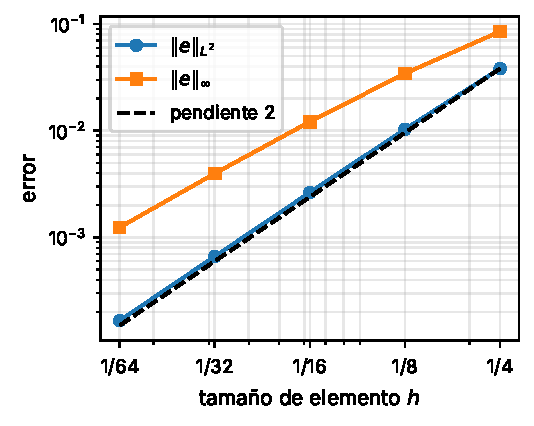
\includegraphics[width=\linewidth]{verificacion_convergencia}
  \caption{Caso 1}
\end{subfigure}\hfill
\begin{subfigure}[b]{0.49\textwidth}
  \centering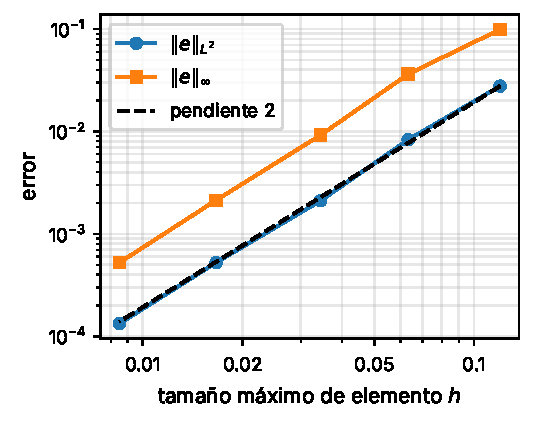
\includegraphics[width=\linewidth]{verificacion_mixta_convergencia}
  \caption{Caso 2}
\end{subfigure}
\caption{Convergencia del error al refinar la malla en los dos casos de verificación.}
\label{fig:verif-conv}
\end{figure}

\begin{figure}[htbp]
\centering
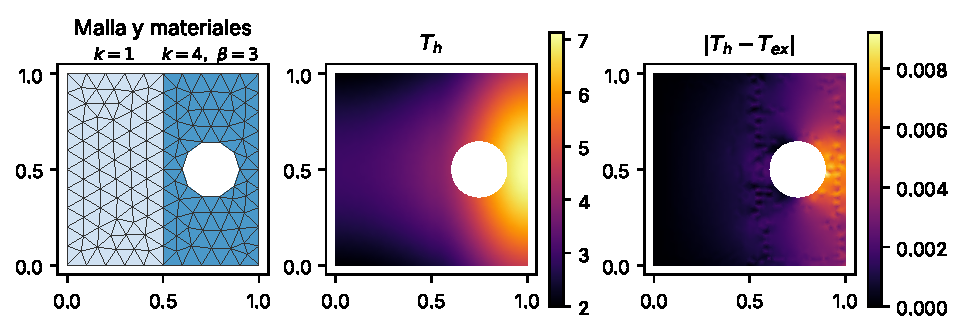
\includegraphics[width=\textwidth]{verificacion_mixta_campos}
\caption{Caso de verificación 2: malla no estructurada más gruesa con los dos materiales,
solución de elementos finitos y error absoluto en la malla de \num{1870} nodos.}
\label{fig:verif-campos}
\end{figure}

La Tabla~\ref{tab:verif} y la Figura~\ref{fig:verif-conv} muestran que el error en $L^2$
converge con orden 2 en ambos casos, como predice la teoría. En el caso 1, el error máximo
nodal converge con un orden algo menor (\num{1.68}), consistente con la cota
$\mathcal O(h^2|\ln h|)$ en norma infinito; el error se concentra en las esquinas, donde se
encuentran dos lados con datos de Robin distintos. En el caso 2, el orden observado fluctúa
entre \num{1.9} y \num{2.3} porque las mallas no estructuradas no se refinan de forma
perfectamente uniforme, pero la tendencia es claramente de orden 2. El agujero se aproxima
con un polígono, cuyo error geométrico también es $\mathcal O(h^2)$ y no degrada la
convergencia. Las pruebas automáticas del repositorio incluyen además una \emph{prueba de
parche}, que comprueba que una solución lineal se reproduce hasta el error de redondeo, y
una prueba de la propiedad de superposición \eqref{eq:superposicion}.

Para mostrar la generalidad del programa fuera del problema del chip, la
Figura~\ref{fig:soporte} resuelve un soporte de aluminio en forma de L
($k=\SI{205}{\watt\per\metre\per\kelvin}$) con un inserto de cobre
($k=\SI{400}{\watt\per\metre\per\kelvin}$) y un canal circular de refrigeración. La base
está en contacto con una pieza a \SI{90}{\celsius} (Dirichlet), el canal transporta agua a
\SI{20}{\celsius} con $h=\SI{2000}{\watt\per\metre\squared\per\kelvin}$ (Robin), el tope
recibe un flujo de \SI{5}{\kilo\watt\per\metre\squared} (Neumann) y el resto intercambia
calor con el aire. Este problema se resuelve solo cambiando la malla y el archivo JSON.

\begin{figure}[htbp]
\centering
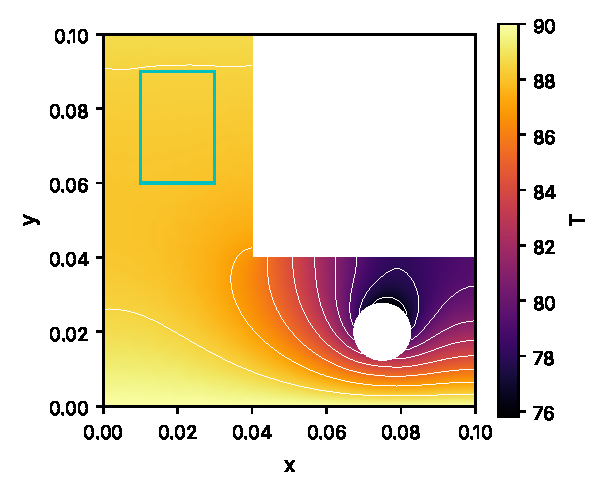
\includegraphics[width=0.62\textwidth]{soporte}
\caption{Ejemplo de generalidad: soporte de aluminio en L con un inserto de cobre (contorno
cian) y un canal de refrigeración, resuelto a partir de archivos de entrada (\num{1986}
nodos). Se combinan condiciones de Dirichlet, Neumann y Robin.}
\label{fig:soporte}
\end{figure}


\subsection{Comparación de las estrategias de disipación}

La Tabla~\ref{tab:resultados} resume los resultados. La primera observación es que, con la
misma capacidad total de enfriamiento, la probabilidad de falla varía en un factor de 18
según cómo se distribuya el disipador: de \num{0.042} con el diseño según potencia pico a
\num{0.755} con el diseño centrado. La ubicación del enfriamiento importa tanto como su
cantidad, en coherencia con la longitud de decaimiento $\lambda\approx\SI{1.9}{\milli\metre}$
de la Sección~\ref{sec:modelo}: el calor se evacúa cerca de donde se genera. El diseño
centrado es el peor porque concentra el enfriamiento sobre la caché, que disipa poco, y deja
la mayor parte de los núcleos y de la GPU con la mitad del coeficiente medio
(Figura~\ref{fig:disenos}). Las estimaciones de Monte Carlo coinciden con los valores
exactos dentro de sus intervalos de confianza en los cuatro diseños, lo que verifica la
implementación del muestreador NORTA. Las frecuencias de activación simuladas reproducen
las $p_i$ objetivo con un error no mayor que \num{0.003}, y la correlación medida entre dos
núcleos vecinos (\num{0.295}) concuerda con la predicha por \eqref{eq:rhoA} (\num{0.297}).

\begin{table}[htbp]
\centering
\caption{Resultados de las cuatro estrategias ($\ell=\SI{3}{\milli\metre}$). $\Pf$ exacta
por enumeración \eqref{eq:enumeracion}; Monte Carlo con $N=\num{2e5}$ e intervalo de Wilson
al 95\,\%. La última columna es el análisis determinista de peor caso.}
\label{tab:resultados}
\small
\setlength{\tabcolsep}{4pt}
\begin{tabular}{@{}lccccc@{}}
\toprule
 & $\Pf$ & $\hat P_N$ & $\mathbb E[\Tmax]$ & Config. & $\Tmax$ todo \\
Estrategia & exacta & [IC 95\,\%] & [\si{\celsius}] & que fallan & encendido [\si{\celsius}] \\
\midrule
Uniforme             & \num{0.451} & \num{0.450} [\num{0.448}, \num{0.453}] & \num{93.0}  & 96/256  & \num{111.9} \\
Centrado             & \num{0.755} & \num{0.755} [\num{0.753}, \num{0.756}] & \num{107.8} & 217/256 & \num{131.6} \\
Según potencia media & \num{0.295} & \num{0.296} [\num{0.294}, \num{0.298}] & \num{86.9}  & 127/256 & \num{106.1} \\
Según potencia pico  & \num{0.042} & \num{0.042} [\num{0.041}, \num{0.043}] & \num{86.4}  & 2/256   & \num{100.5} \\
\bottomrule
\end{tabular}
\end{table}

La última columna de la Tabla~\ref{tab:resultados} muestra la limitación del análisis de
peor caso. Con todos los bloques encendidos, las cuatro estrategias superan
$\Tc=\SI{100}{\celsius}$, de modo que un criterio determinista las declararía a todas
inaceptables y no las podría ordenar. El diseño según potencia pico supera el límite por
apenas \SI{0.5}{\celsius} y solo en 2 de las 256 configuraciones, lo que en la práctica
corresponde a una probabilidad de falla de \SI{4}{\percent}, frente a \SI{45}{\percent} del
diseño uniforme. La diferencia entre ambos, estimada con números aleatorios comunes, es
$\num{0.409}\pm\num{0.002}$.

El resultado más llamativo es la comparación entre los diseños según potencia media y según
potencia pico. Sus temperaturas máximas esperadas son casi iguales (\SI{86.9}{\celsius}
frente a \SI{86.4}{\celsius}), pero sus probabilidades de falla difieren en un factor de
siete. La causa está en la GPU: tiene la segunda mayor densidad de potencia, pero se usa
poco ($p=\num{0.3}$), así que el diseño según potencia media le asigna poco enfriamiento.
En ese diseño fallan 127 de las 128 configuraciones con la GPU encendida y ninguna con la
GPU apagada; por eso su $\Pf$ es prácticamente igual a $p_{\mathrm{GPU}}=\num{0.3}$.
Diseñar para el promedio optimiza la temperatura típica pero deja sin protección los
eventos poco frecuentes de alta potencia, y la temperatura esperada, por sí sola, no revela
ese riesgo.

\begin{figure}[htbp]
\centering
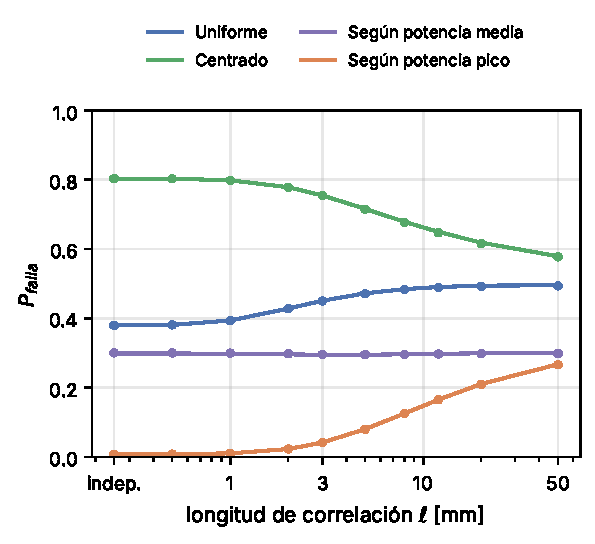
\includegraphics[width=0.68\textwidth]{fig_pfalla_ell}
\caption{Probabilidad de falla en función de la longitud de correlación $\ell$. Las líneas
son el valor exacto y los puntos la estimación de Monte Carlo con intervalos de Wilson al
95\,\% (más pequeños que los marcadores). ``indep.'' corresponde a $\ell=0$.}
\label{fig:ell}
\end{figure}

\subsection{Efecto de la correlación entre bloques}

La Figura~\ref{fig:ell} muestra $\Pf$ en función de la longitud de correlación. El efecto
de la correlación depende del diseño, y se entiende a partir de los casos límite. Cuando
$\ell\to\infty$, todas las variables latentes son iguales y los bloques se encienden en un
orden fijo, de mayor a menor $p_i$, de modo que solo quedan $N_b+1$ configuraciones
posibles, anidadas entre sí. La probabilidad de falla tiende entonces a la probabilidad
de alcanzar la primera configuración de esa secuencia que falla. Por eso las curvas se
aproximan entre sí (entre \num{0.27} y \num{0.58} con $\ell=\SI{50}{\milli\metre}$) y las
diferencias entre diseños se reducen.
\begin{itemize}
\item En el \textbf{diseño según potencia pico}, la falla es un evento raro que exige
  muchos bloques encendidos a la vez. La correlación hace más probables esas coincidencias:
  $\Pf$ pasa de \num{0.008} con bloques independientes a \num{0.042} con
  $\ell=\SI{3}{\milli\metre}$ y a \num{0.27} con $\ell=\SI{50}{\milli\metre}$, es decir,
  aumenta más de 30 veces.
\item En el \textbf{diseño centrado}, la falla es común y basta con pocos bloques
  encendidos. La correlación aumenta la probabilidad de que haya pocos bloques encendidos,
  y $\Pf$ disminuye de \num{0.80} a \num{0.58}.
\item En el \textbf{diseño según potencia media}, $\Pf$ casi no cambia, porque depende solo
  de que la GPU esté encendida, y la probabilidad marginal de un bloque no depende de
  $\ell$.
\end{itemize}

La implicación práctica es importante: suponer bloques independientes, que es la hipótesis
más simple, subestima en un orden de magnitud el riesgo del mejor diseño si la carga real
es correlacionada, como ocurre con programas paralelos que usan todos los núcleos al mismo
tiempo.

\begin{figure}[htbp]
\centering
\begin{subfigure}[b]{0.49\textwidth}
  \centering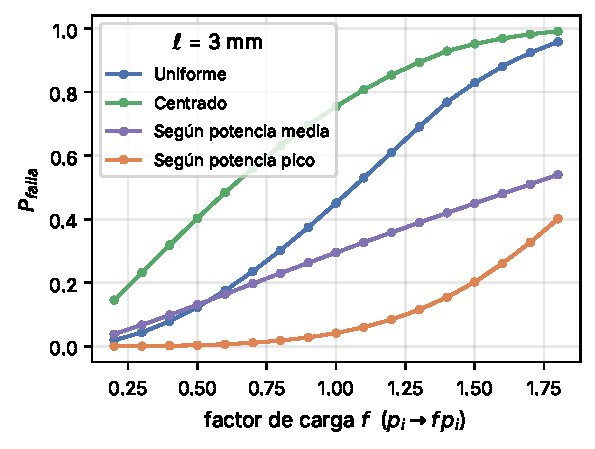
\includegraphics[width=\linewidth]{fig_pfalla_p}
  \caption{Sensibilidad al nivel de carga}
  \label{fig:carga}
\end{subfigure}\hfill
\begin{subfigure}[b]{0.49\textwidth}
  \centering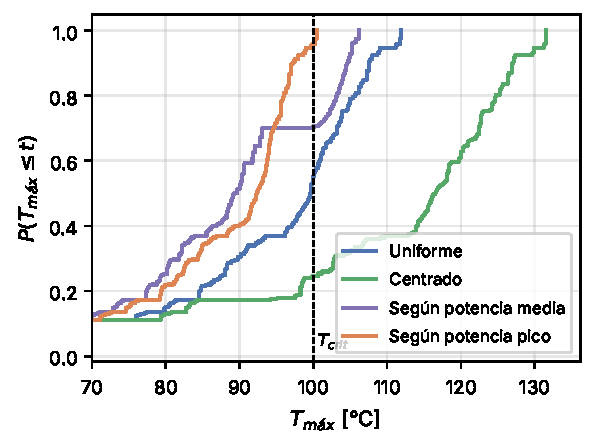
\includegraphics[width=\linewidth]{fig_cdf_tmax}
  \caption{Distribución de $\Tmax$}
  \label{fig:cdf}
\end{subfigure}
\caption{(a) $\Pf$ cuando todas las probabilidades de activación se escalan por un factor
de carga $f$, con $p_i\to\min(f\,p_i,\ \num{0.99})$. La zona sombreada ($f>\num{1.41}$) indica que alguna probabilidad está truncada. (b) Función de distribución acumulada de la temperatura
máxima para $f=1$; la línea discontinua es $\Tc$.}
\label{fig:carga-cdf}
\end{figure}

\subsection{Sensibilidad al nivel de carga y distribución de la temperatura máxima}

La Figura~\ref{fig:carga} escala todas las probabilidades de activación por un factor
$f$, que representa usos más livianos ($f<1$) o más intensos ($f>1$) del chip. Como una
probabilidad no puede superar 1, las probabilidades escaladas se truncan:
\begin{equation}
  p_i' = \min\!\left(f\,p_i,\ \num{0.99}\right).
  \label{eq:truncamiento}
\end{equation}
El tope es \num{0.99} y no 1 porque con $p_i'=1$ el umbral de \eqref{eq:norta} sería
$c_i=\Phi^{-1}(0)=-\infty$: el bloque dejaría de ser aleatorio y las probabilidades de los
ortantes quedarían mal definidas. En el rango estudiado ($f\le\num{1.8}$) el truncamiento
solo afecta a dos bloques: la caché L3 ($p=\num{0.7}$), que se satura a partir de
$f\approx\num{1.41}$, y el controlador de memoria ($p=\num{0.6}$), a partir de
$f=\num{1.65}$. Los núcleos, la GPU y la E/S nunca se saturan. Por tanto, para $f>\num{1.41}$
el escalamiento deja de ser uniforme y la parte derecha de la figura debe leerse con esa
salvedad; las conclusiones se apoyan en el rango $f\le\num{1.4}$, donde no hay truncamiento. El diseño
según potencia pico es el mejor en todo el rango, pero el orden entre los otros dos no es
fijo: con carga baja ($f\lesssim\num{0.55}$), el diseño según potencia media es
\emph{peor} que el uniforme, y con carga alta es mejor. Esto refuerza la idea central del
trabajo: qué diseño conviene depende del uso esperado del chip, y esa dependencia solo se
observa con un modelo probabilístico de la carga.

La Figura~\ref{fig:cdf} muestra la distribución completa de $\Tmax$. Como hay un número
finito de configuraciones, la distribución es escalonada. La curva del diseño según
potencia media tiene un salto grande justo por encima de $\Tc$, que corresponde a las
configuraciones con la GPU encendida; la del diseño según potencia pico queda casi entera a
la izquierda de $\Tc$.

\begin{figure}[htbp]
\centering
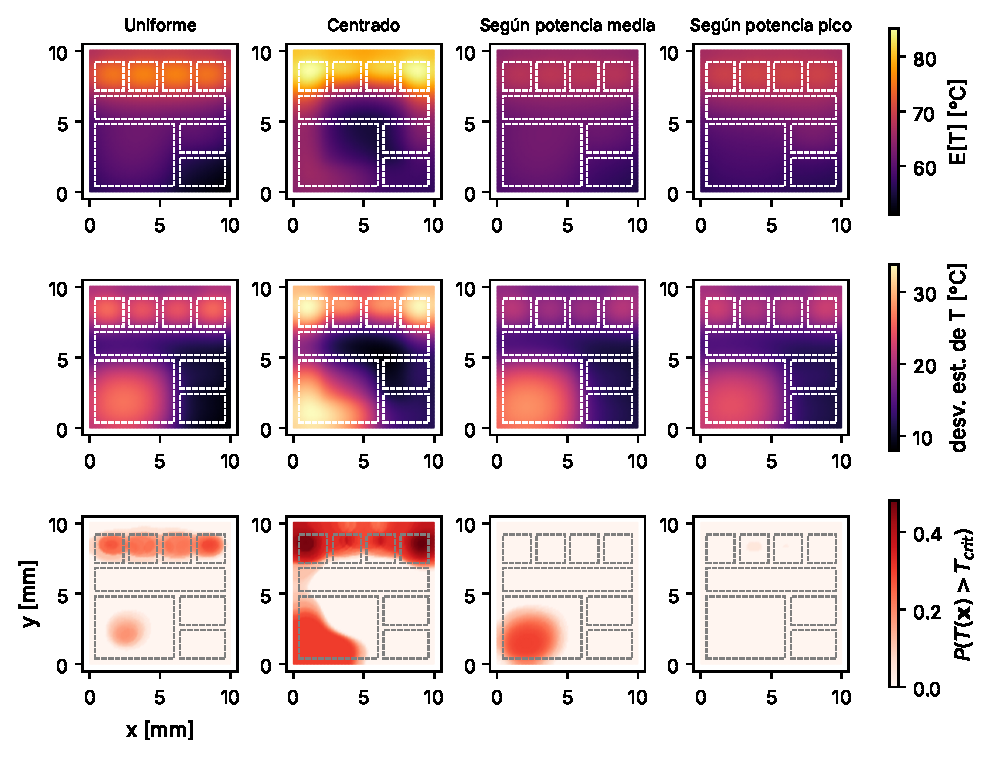
\includegraphics[width=\textwidth]{fig_mapas}
\caption{Campos estadísticos exactos para $\ell=\SI{3}{\milli\metre}$: temperatura media
(arriba), desviación estándar de la temperatura (centro) y probabilidad puntual
$P(T(\vec x)>\Tc)$ (abajo).}
\label{fig:mapas}
\end{figure}

\subsection{Distribución espacial del riesgo}

La Figura~\ref{fig:mapas} muestra dónde se concentra el riesgo en cada diseño. La
desviación estándar de la temperatura es mayor sobre la GPU y los núcleos, los bloques con
más potencia y mayor varianza de activación, $p_i(1-p_i)$. El mapa de probabilidad puntual
identifica las zonas que causan las fallas: los núcleos y, en menor medida, la GPU en el
diseño uniforme; ambas zonas en el diseño centrado; solo la GPU en el diseño según potencia
media; y apenas un punto en el núcleo 2 en el diseño según potencia pico. Estos mapas son útiles para el diseño porque muestran dónde
conviene añadir capacidad de enfriamiento y no solo cuánta.

\subsection{Convergencia de las estimaciones}
\label{sec:convergencia}

\begin{figure}[htbp]
\centering
\begin{subfigure}[b]{0.40\textwidth}
  \centering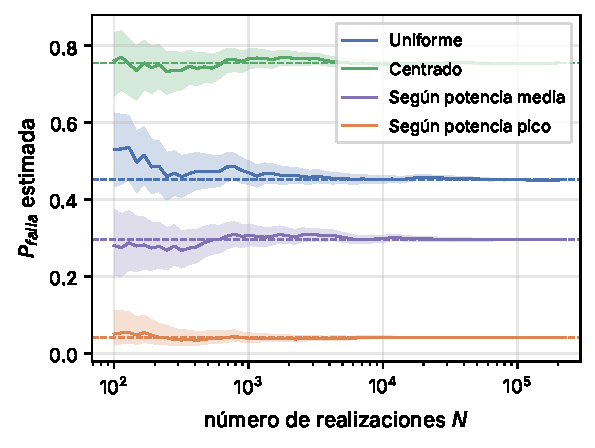
\includegraphics[width=\linewidth]{fig_convergencia_mc}
  \caption{Monte Carlo}
  \label{fig:conv-mc}
\end{subfigure}\hfill
\begin{subfigure}[b]{0.58\textwidth}
  \centering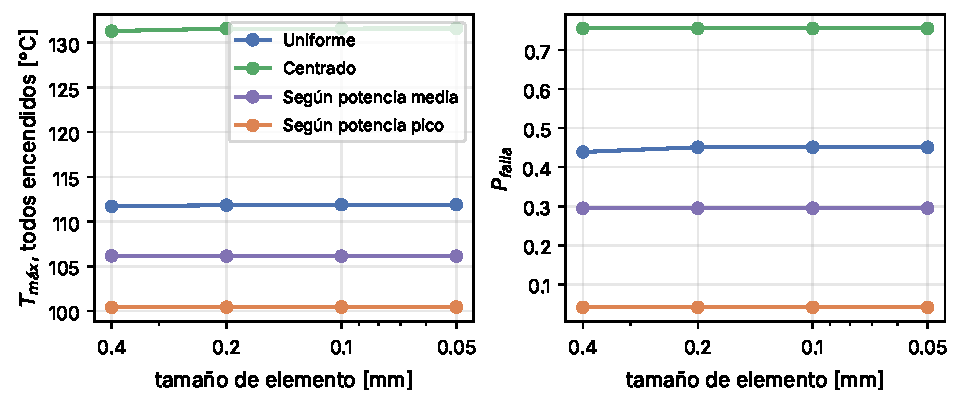
\includegraphics[width=\linewidth]{fig_convergencia_malla}
  \caption{Malla}
  \label{fig:conv-malla}
\end{subfigure}
\caption{(a) Estimación de Monte Carlo en función del número de realizaciones, con bandas
de Wilson al 95\,\%; las líneas discontinuas son los valores exactos. (b) $\Tmax$ con todos
los bloques encendidos y $\Pf$ en función del tamaño de elemento.}
\label{fig:convergencia}
\end{figure}

La Figura~\ref{fig:conv-mc} muestra que la estimación de Monte Carlo se estabiliza
alrededor del valor exacto y que el ancho de la banda de confianza decrece como $N^{-1/2}$.
Para $N=\num{2e5}$, el semiancho del intervalo es de \numrange{0.001}{0.002}, muy inferior a
las diferencias entre diseños. Los números aleatorios comunes reducen la varianza de la
diferencia entre diseños en un factor de \numrange{1.2}{1.9}, según el par comparado y el
plano de bloques; la reducción es modesta aquí porque los diseños fallan en
configuraciones distintas, lo que debilita la correlación entre sus indicadores.

En cuanto a la malla (Figura~\ref{fig:conv-malla}), la temperatura máxima con todos los
bloques encendidos cambia menos de \SI{0.02}{\celsius} entre las mallas de $100^2$ y $200^2$
celdas. $\Pf$ es una función discontinua de la malla, porque una configuración con $\Tmax$
muy cercana a $\Tc$ puede cambiar de lado al refinar. Así ocurre en el diseño uniforme entre
$25^2$ y $50^2$ celdas, donde $\Pf$ pasa de \num{0.439} a \num{0.451}. A partir de la malla
de $50^2$, $\Pf$ no cambia en ninguno de los cuatro diseños, de modo que el error de
discretización es despreciable frente al de muestreo en la malla de $100^2$ usada.

\subsection{Caso idealizado de bloques iguales}

Como referencia, el estudio se repitió con el plano de la entrega de avance: nueve bloques
iguales de \SI{2}{\milli\metre}, de \SI{13}{\watt} cada uno y con $p=\num{0.5}$. En ese caso
los diseños según potencia media y según potencia pico coinciden exactamente, porque todos
los bloques tienen la misma potencia y la misma probabilidad, y se obtiene
$\Pf=\num{0.168}$ frente a \num{0.449} del diseño uniforme. La tendencia con $\ell$ es la
misma: $\Pf$ crece de \num{0.049} a \num{0.42} en el mejor diseño. El caso idealizado
reproduce el efecto de la correlación, pero no puede mostrar la diferencia entre diseñar
para la media y para el pico, que aparece solo cuando los bloques son heterogéneos. Esto
justifica el uso de un plano realista.

% =============================================================================
\section{Conclusiones}
\label{sec:conclusiones}

Se desarrolló un solver propio de elementos finitos lineales para la ecuación de
Helmholtz modificada con varios materiales y condiciones de Dirichlet, Neumann y Robin,
configurable mediante archivos de entrada. Se verificó con dos soluciones manufacturadas,
una de ellas en mallas no estructuradas con interfaz entre materiales y condiciones
mixtas, alcanzando el orden 2 esperado en norma $L^2$. Con él se estudió el riesgo de
sobrecalentamiento de un chip cuya carga de trabajo es aleatoria y correlacionada. Las
principales conclusiones son:
\begin{enumerate}
\item Con la misma capacidad total de enfriamiento, la distribución espacial del
  disipador cambia la probabilidad de falla entre \num{0.04} y \num{0.75}. Dónde se enfría
  importa tanto como cuánto se enfría.
\item El análisis de peor caso no permite comparar estrategias: las cuatro superan el
  límite con todos los bloques encendidos, aunque sus probabilidades de falla difieren en un
  factor de 18.
\item Diseñar según la potencia media produce casi la misma temperatura máxima esperada
  que diseñar según la potencia pico, pero una probabilidad de falla siete veces mayor,
  porque desprotege los bloques potentes de uso poco frecuente. La temperatura esperada no
  es un buen indicador de riesgo.
\item La correlación espacial de la carga aumenta el riesgo de los buenos diseños, más de
  30 veces en el mejor caso estudiado, y reduce el de los malos. Suponer independencia
  puede subestimar gravemente el riesgo real.
\item El orden entre estrategias depende del nivel de carga, por lo que el diseño del
  disipador debe tener en cuenta el uso esperado del chip.
\end{enumerate}
Desde el punto de vista numérico, la linealidad del problema permitió reducir cada
realización a una suma de vectores y calcular la probabilidad de falla de forma exacta por
enumeración. Monte Carlo, verificado contra ese valor exacto, queda como la herramienta
para planos con muchos más bloques.

\paragraph{Limitaciones y trabajo futuro} El modelo es bidimensional y estacionario: supone
que cada configuración de actividad dura más que la constante de tiempo térmica del chip,
y resume todo el camino hacia el aire en un único coeficiente $\hs$. Las potencias y
probabilidades de activación son supuestos representativos, no mediciones de un procesador
concreto, y la correlación solo depende de la distancia, cuando en la práctica también
depende de la función de los bloques. La cópula gaussiana no tiene dependencia en las
colas, por lo que podría subestimar la frecuencia de activaciones extremas simultáneas.
Como trabajo futuro se proponen: un modelo transitorio con la ecuación del calor, el uso de
trazas de potencia medidas para calibrar $p_i$ y $\Sigma$, la optimización de $\hs$ para
minimizar $\Pf$ con la capacidad total fija, y la validación del modelo con mediciones
experimentales o con un simulador de referencia como HotSpot \cite{huang2006hotspot}.

% =============================================================================
\section*{Disponibilidad del código}
\label{sec:codigo}
El código fuente, las mallas, los archivos de entrada, las pruebas automáticas y los
scripts que reproducen todas las figuras y tablas están disponibles en
\url{https://github.com/marioarroyaveaguirre2004-boop/proyecto-metodos-edp-Grupo6}. Cada figura se regenera con un solo comando y
semilla fija.

\section*{Declaración sobre el uso de inteligencia artificial}
Durante este trabajo los autores usaron un asistente de inteligencia artificial generativa
(Claude, de Anthropic) como apoyo en el desarrollo y la depuración de partes del código, en
la generación de figuras y en la redacción de borradores del texto. Los autores revisaron,
ejecutaron y verificaron todo el código y los resultados, y editaron el contenido. Asumen
total responsabilidad por el contenido de esta publicación.

\bibliographystyle{elsarticle-num}
\bibliography{referencias}

\end{document}
